\vspace{-2mm}
\section{FKM Richtlinien}{}
    \subsection{Auslastungsgrad}
     
        \subsubsection{Definitionen}
            \begin{enumerate}[noitemsep]
                \item $\sigma_{v}$: Vergleichsspannung im Nachweispunkt
                \item $\sigma_{SK}$: Materialfestgkeit, bauteilspezifisch
                \item $J_{ges}$: Sicherheitsfaktor (Gesamtsicherheitsfaktor)
            \end{enumerate}
            \vspace{-1mm}\[a_{SK} = \frac{\sigma_{v}}{\sigma_{sk}/J_{ges}} \]
    
        \subsubsection{Mehrachsigkeit}
            Falls $h > 1.33$ zusätzlicher Nachweis erforderlich! (Bruchdehnung und ev. maximale äquivalente Spannung bei starker Mehrachsigkeit kleiner)
            \vspace{-2mm}\[ h = \frac{\frac{1}{3} \textrm{Spur}[T]}{\sigma_{\textrm{v. Mises}}} \quad \textrm{[T]: Spannungstensor}\]
        \subsubsection{Bauteilfestigkeit $\sigma_{\textrm{SK}}$}
            An Normprobe gemessene Fliessgrenze erffordert meistens Korrektur! \\$R_P$: Fliessgrenze Bauteil; $R_{P,N}$: Fliessgrenze Normprobe.
            \vspace{-2mm}
            \[R_P = K_{d,P}\cdot K_A\cdot R_{P,N}\]
            \vspace{-4mm}
            \[\sigma_{\textrm{SK}}=R_p\cdot n_{\textrm{pl}} \quad\textrm{mit: } \small n_{\textrm{pl}}=\textrm{min} \left( \sqrt{ \frac{E\cdot\varepsilon_{\textrm{ertr}}}{R_p}};K_p \right) \quad \sigma_v^{el}\frac{\sigma_v^{el}}{E}=R_p\cdot\varepsilon_{\textrm{ertr}}\]\normalsize
            Hom. Spannungsverteilung: $n_{\textrm{pl}}=1$ (Keine Reserve)
            \vspace{-1mm}
            \[K_p: \textrm{pl. Formzahl} = \frac{\textrm{Last beim Versagen 
            (bspw vMises)}}{\textrm{Last bei erster Plast}}\]
            vollpl.: aus FE; el. Grenzl.: wenn $\sigma_v = R_p$ erreicht.
        \subsubsection{Sicherheitsfaktor $J_{\textrm{ges}}$}
        \small\[J_{\textrm{ges}}= J_s \cdot \left[ J_z \cdot \textrm{max}\left(\frac{J_m \cdot R_p}{R_m}; J_p \right) \right] \]\normalsize
        $J_s$: Lastfaktor (Sicher:=1); $J_z$: Schweissteile; $J_p$: plastifizierung
        \begin{center}
            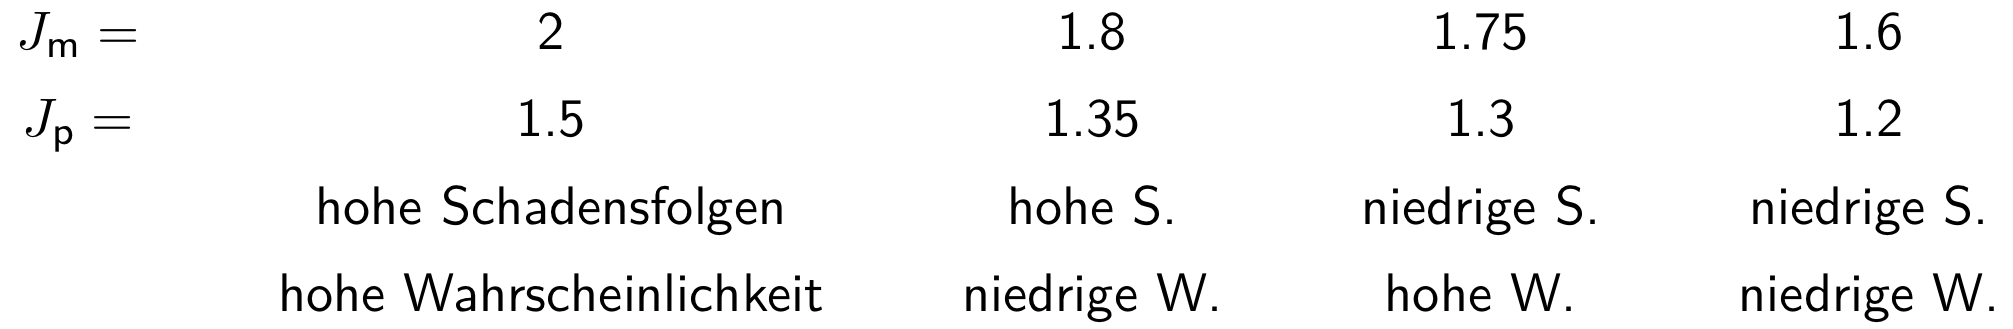
\includegraphics[width=0.8\linewidth]{05/Sicherheitsfaktoren.png}
        \end{center}
    
    \subsection{BSP}
        \subsubsection{plastische Formzahl an einem Druckkessel mit Loch}
            \begin{enumerate}
                \item Loch belastet mit $2s,s$ wobei $s=\sigma_{zz}$ $\rightarrow$ kritische Stelle $=5s$
                \item $R_e=5s=5\sigma_{zz}=\frac{5R}{2d}P \Leftrightarrow P_{pl}=\frac{2d}{5R}R_e=:$Last bei erster Plast.
                \item Versagenslast: $R_e=\sigma_{v.Mises}^{vgl}(\sigma_{rr},\sigma_{\varphi\varphi},\sigma_{zz})=\frac{\sqrt{3}R}{2d}R_e \Leftrightarrow P_{vers}=\frac{2d}{\sqrt{3}R}R_e$
                \item $K_p=\frac{P_{vers}}{P_{pl}}\approx 2.88$
            \end{enumerate}
            
        \subsubsection{Dimensionieren eines Kessels mit Loch nach FKM}
        Ziel: $ a_{SK}<1 $
        \\\textit{Vorgehen:}
        \vspace{-3mm}
        \begin{enumerate}
            \item $ a_{{SK}} = \frac{\frac{\sigma_v}{\sigma_{{SK}}}}{J_{ges}}  \rightarrow  \sigma_v \cdot J_{ges} < \sigma_{{SK}} $
            \item Wegen Mehrachsigkeit kein weiterer Nachweis nötig
            $ h = \frac{1}{3} < 1.33$ 
            \item Bauteilspezifische Materialfestigkeit $ \sigma_{SK} $ berechnen:
            \item Sicherheitsfaktor $J_{ges}$ berechnen
            \item Einsetzen in 1. ergibt $a_{SK}=0.4<1$
        \end{enumerate}
        
        
        
        
        
        
        
